\chapter{PyEvoMotion: a software to perform the temporal statistical analysis of genome evolution}

\begin{flushright}
    \textit{One accurate measurement is worth a thousand expert opinions.}\\
    --- Grace Hopper
\end{flushright}

\vspace{1cm}

\noindent This work has been sent to a peer-reviewed journal.\\

\noindent \textbf{Goiriz L}, Rodrigo G. (2025) {PyEvoMotion: a software to perform the temporal statistical analysis of genome evolution}. \textit{Under review}.\\

\noindent In this publication, I performed all the software development, testing and documentation. The results were discussed with GR. GR designed the research.

\vfill

\pagebreak

\sloppy

\section{Introduction}

The study of molecular evolution is a central topic in biology. The molecular clock hypothesis assumes that genes accumulate mutations at a constant rate over time \cite{kimura1987}. Moreover, under the consideration that most of the accumulated mutations are neutral, the Poisson distribution models the expected variability. The molecular clock hypothesis has become a cornerstone of modern phylogenetic techniques, which are now standard for studying the evolutionary relationships between species and organisms \cite{kumar2005}.

It has been shown, however, that the simple molecular clock model fails to universally recapitulate evolutionary trajectories. Observations revealed that in some cases mutations do not accumulate at a constant rate \cite{ayala1997}. This led to the development of relaxed molecular clocks, in which the rates of mutation accumulation are not uniform across lineages \cite{drummond2008}. Although these clocks have proven to be more accurate in certain cases, they still face difficulties to model, for instance, overdispersed populations \cite{bedford2008}. A proper analysis of the time-dependent distribution of the number of mutations in the population is necessary to understand and eventually predict the evolutionary trajectories that take place in nature.

Although previous studies have attempted to abstract molecular evolution as a type of diffusion process in the sequence space \cite{kimura1987, huynen1996}, little attention has been given to the form of the underlying stochastic process. In our previous work, we showed that non-Brownian evolutionary motions occurred within the lineages of a virus, leading to non-Poissonian distributions \cite{goiriz2023}. Here, we present PyEvoMotion, a Python tool aimed to infer a generalized molecular clock model upon bulk genomic data analysis, featuring a command-line interface and enough modularity for integration into larger Python pipelines. PyEvoMotion is intended to complement traditional phylogenetic analyses.

Traditional phylogenetic methods, while powerful, face computational limitations when applied to large datasets. Indeed, analyzing more than $10^4$ sequences becomes impractical due to the exponential complexity of reconstructing evolutionary trees \cite{chor2005}. To overcome this bottleneck, statistical approaches provide a viable alternative \cite{goiriz2023, obermeyer2022}. These methods simplify the representation of evolutionary relationships by focusing on patterns of population genetics rather than exhaustive tree reconstruction based on genetic variation. PyEvoMotion leverages stochastic mathematical modelling to assess evolutionary trends, aiming to process datasets orders of magnitude larger than those typically analyzed. This capability is essential for handling the unprecedented volume of genomic data generated by high-throughput sequencing efforts \cite{oude2020}.

\section{Implementation}

\subsection{Data processing}
The general workflow of PyEvoMotion is illustrated in Figure~\ref{fig1:pyevomotion_overview}. This tool requires two essential input files: a \texttt{.fasta} file containing nucleic acid sequences and a \texttt{.tsv} file with the corresponding metadata. Users can customize their analyses by specifying several parameters and filters.
\begin{figure*}[h!]
    \centering
    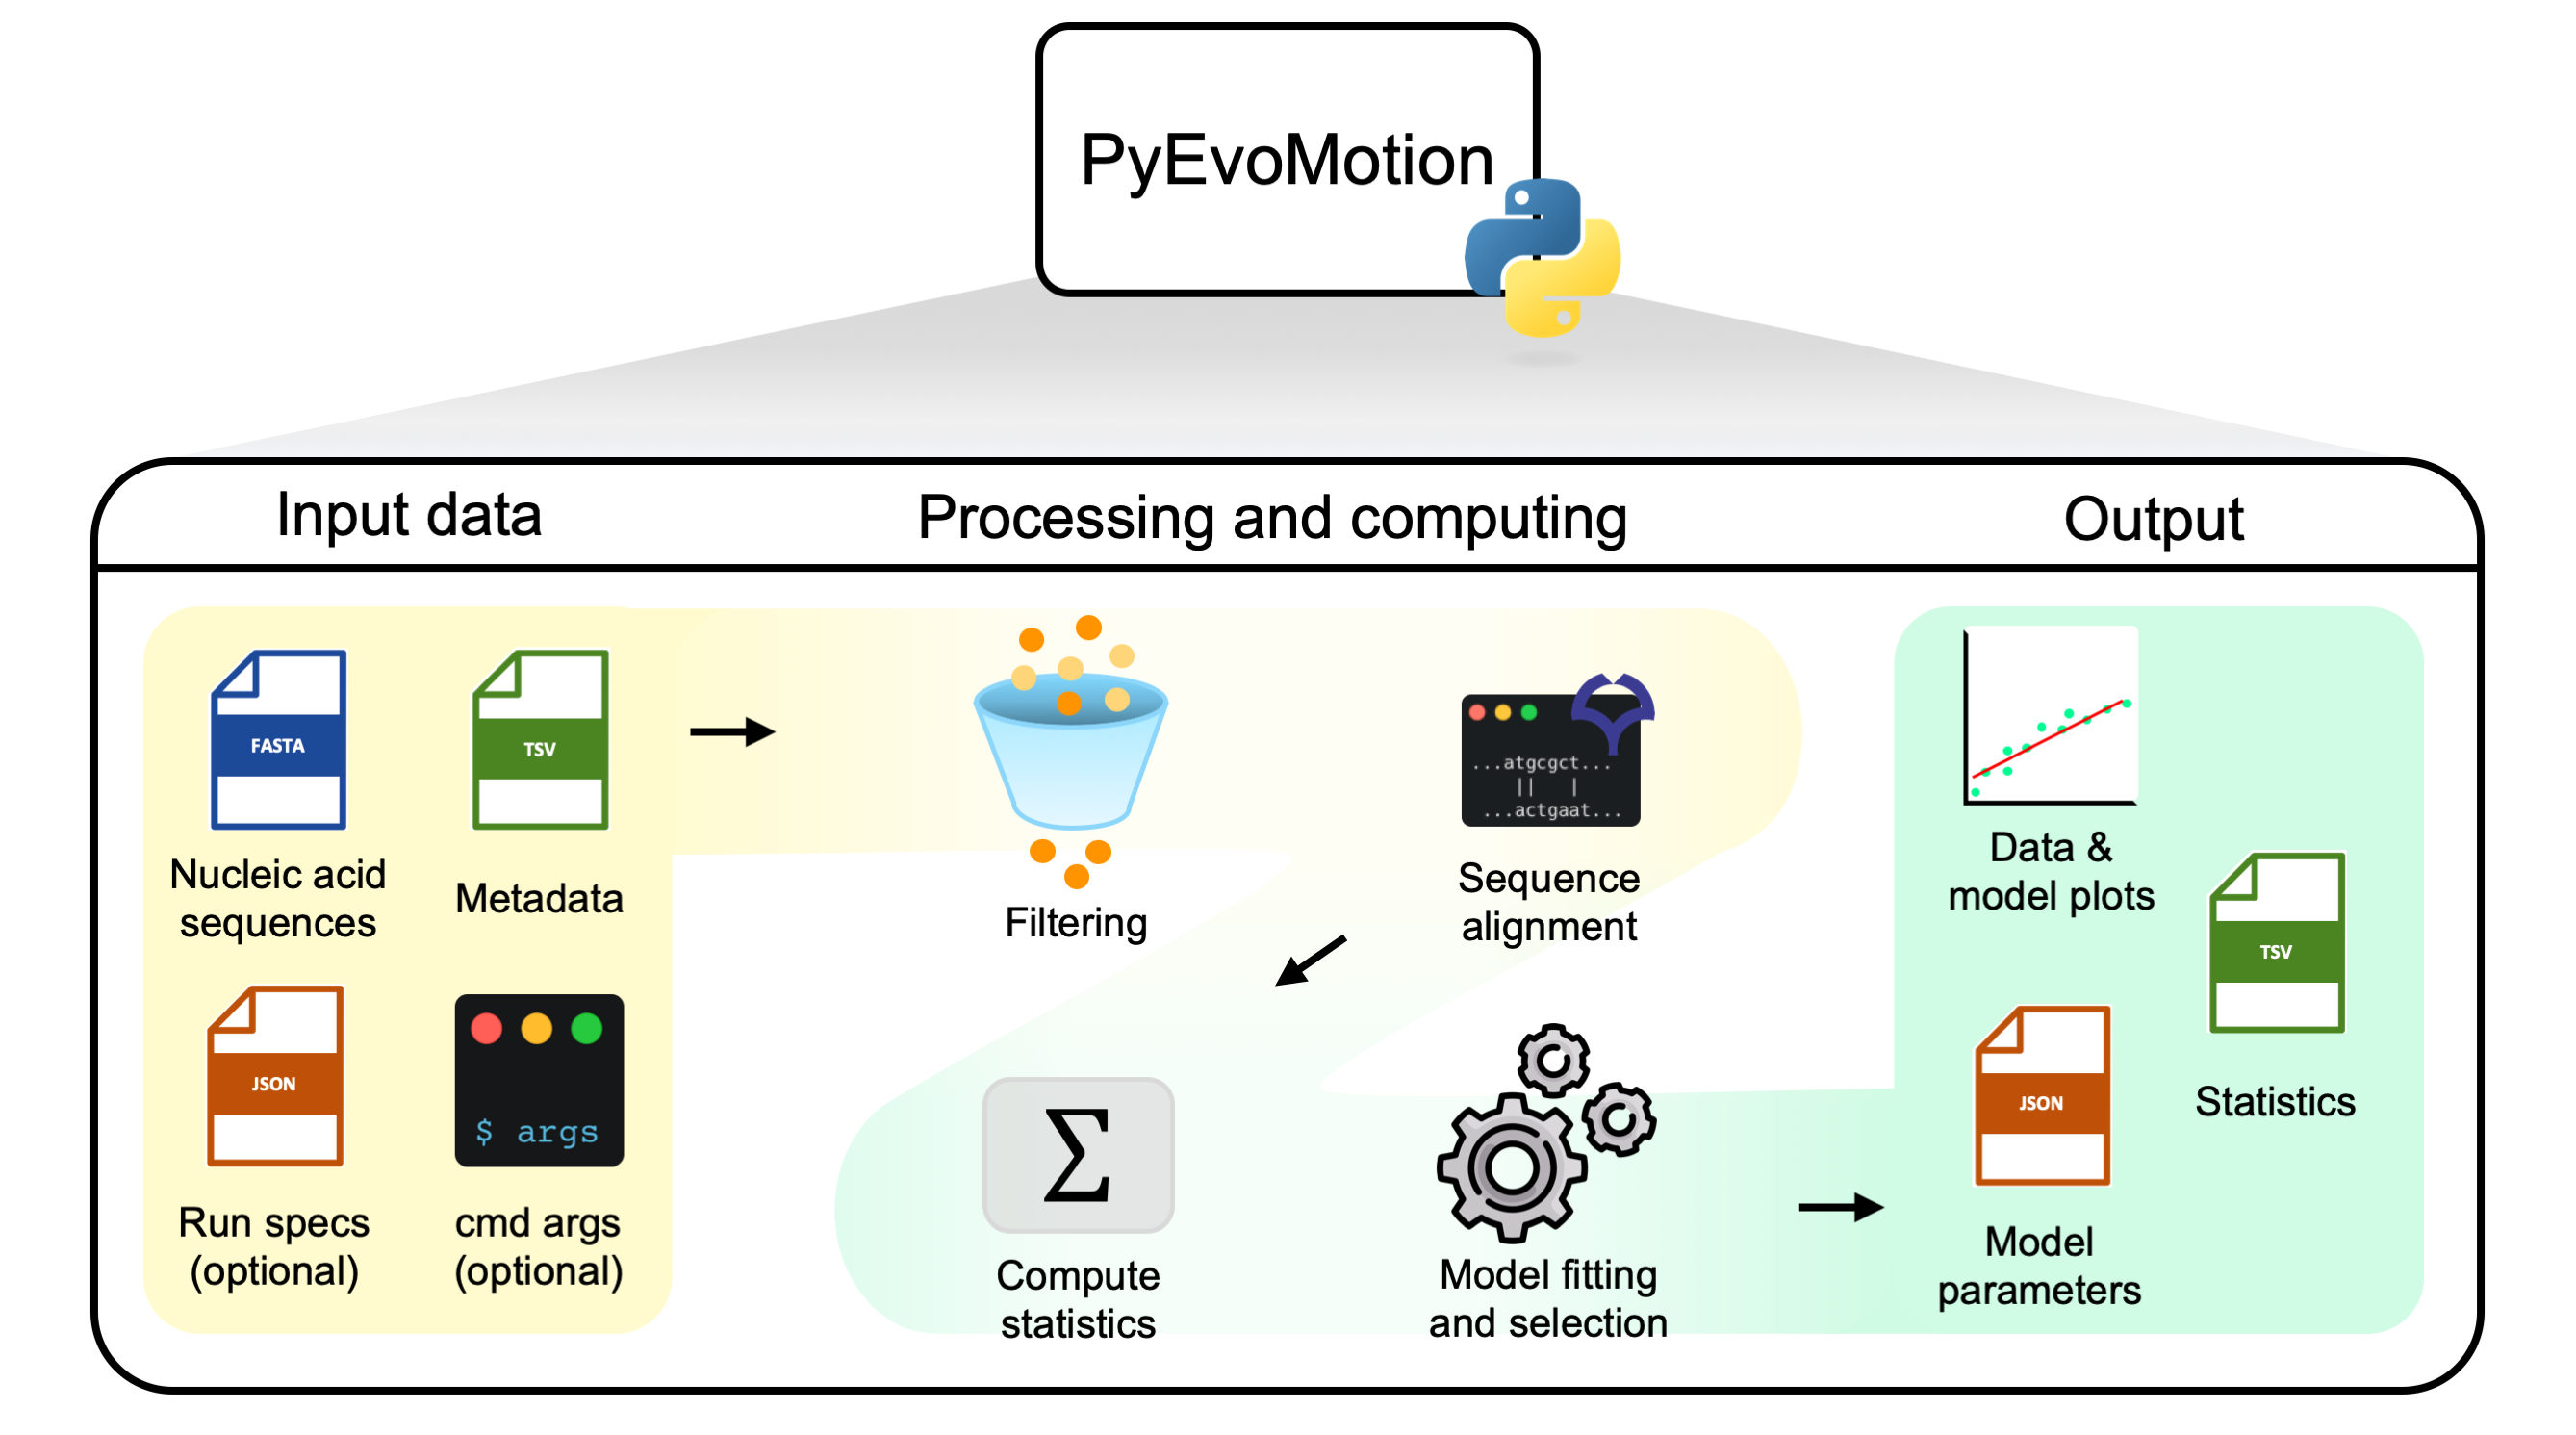
\includegraphics[trim={0 0.3cm 0 0},clip,width=0.9\textwidth]{assets/Ch3Fig1.png}
    \caption{Overview of PyEvoMotion. Mandatory input data include nucleic acid sequences (in \texttt{.fasta} format) and their corresponding metadata (in \texttt{.tsv} format). The metadata must include collection dates, as these are essential for model fitting. Output files include dynamic data representation plots and statistical parameters.}\label{fig1:pyevomotion_overview}
\end{figure*}

To begin, the temporal granularity of the analysis can be adjusted by defining the time intervals for grouping sequences and calculating statistics. By default, this interval is set to 7 d. Additionally, data filtering options are available to enhance the quality and specificity of the analysis. For instance, the length filter excludes sequences that do not meet a minimum length threshold, thereby removing low-quality genomes (unresolved bases set to a maximum of 1\% \texttt{N}). The genome position filter allows users to restrict the analysis to specific genomic regions, which is particularly useful for examining genes or genetic clusters of interest. A date range filter further refines the dataset by limiting the analysis to sequences collected within a specified timeframe.

The tool also enables users to select the types of mutations to include in the analysis. Options include: \texttt{total} (aggregating all mutations without distinction), \texttt{substitutions}, and \texttt{indels} (a combined category of insertions and deletions). These three analyses can be done at once with the option \texttt{all}. Filters based on metadata values provide additional flexibility, enabling users to focus on sequences that meet specific criteria in their non-molecular attributes.

After parsing the sequence data, the reference sequence is extracted, defined as the first entry in the \texttt{.fasta} file. Following the pre-processing step, each sequence is aligned to the reference sequence using the MAFFT algorithm \cite{katoh2013}. Below is an excerpt from PyEvoMotion's \texttt{parser.py} source file showing how MAFFT is invoked as a subprocess via the \texttt{\_run\_mafft()} class method, which directly communicates with the MAFFT executable via binary pipes. The \texttt{generate\_alignment()} class method takes two strings, invokes \texttt{\_run\_mafft()}, retrieves the aligned output binary data, and parses it via Biopython's \texttt{AlignIO}, ensuring precise, high-throughput alignment of genomic data prior to mutation detection:

\begin{lstlisting}[language=Python, caption={Calling MAFFT for sequence alignment.}]
@classmethod
def generate_alignment(cls, seq1: str, seq2: str) -> MultipleSeqAlignment:
"""
Generate a multiple sequence alignment of the input sequences using ``MAFFT``.

:param seq1: The first sequence to be aligned.
:type seq1: str
:param seq2: The second sequence to be aligned.
:type seq2: str
:return: The aligned sequences.
:rtype: ``MultipleSeqAlignment``
"""

id_1 = seq1.id
id_2 = seq2.id

if seq1.id == seq2.id:
    id_1 += "_ref"

return AlignIO.read(
    StringIO(cls._run_mafft({
        id_1: seq1.seq,
        id_2: seq2.seq
    })),
    "fasta"
)

@staticmethod
def _run_mafft(seqs_dict: dict[str,str], outformat: str = "fasta") -> str:
    """
    This function runs the MAFFT multiple sequence alignment tool on the input sequences.

    It raises an exception if the return code is not 0 (i.e. there was an error running MAFFT).

    :param seqs_dict: A dictionary containing the sequences to be aligned. The keys are the sequence
                      names and the values are the sequences.
    :type seqs_dict: dict[str,str]
    :param outformat: The output format of the alignment. Default is fasta.
    :type outformat: str
    :return: The aligned sequences as parsed from stdout. If the output format is clustal, it returns
             the alignment in clustal format; otherwise, it returns the alignment in fasta format.
    :rtype: str
    """

    cmd = ["mafft"]
    template_format = ">{}\n{}\n"

    if outformat == "clustal":
        cmd.extend(["--clustalout", "-"])

    elif outformat != "fasta":
        print(f"Unknown output format: {outformat}. Defaulting to fasta.")

    cmd.append("-")

    input_data = bytes(
        "".join(
            template_format.format(name, seq)
            for name, seq in seqs_dict.items()
        ),
        "utf-8"
    )

    ps = Popen(
        cmd,
        stdin=PIPE,
        stdout=PIPE,
        stderr=PIPE,
        shell=False
    )
    ps.stdin.write(input_data)
    ps.stdin.close()

    err = ps.stderr.read().decode("utf-8")
    out = ps.stdout.read().decode("utf-8")

    if (ps.returncode != 0) and not(ps.returncode is None):
        raise Exception(
            f"Error running MAFFT:\nStdout:\n{out}\n\nStderr:\n{err}\nReturn code: {ps.returncode}"
        )

    return out
\end{lstlisting}

Mutation events are identified from the sequence alignments and filtered based on the user-defined mutation types and genomic regions of interest. The model follows the methodology presented in Chapter \ref{ch:chapter2}, employing a stochastic differential equation that describing the accumulation of mutations over time. The simpler model assumes Gaussian white noise, leading to a scenario where the average number of mutations grows linearly and the variability scales directly with time, resembling Brownian motion. An alternative, more complex model introduces time-dependent noise characterized by a diffusion exponent, resulting in a fractional Brownian motion where the variance scales nonlinearly; both models converge when the diffusion exponent is 1, aligning with the neutral theory of molecular evolution. Statistical analyses are then conducted on the filtered mutation data for each time interval specified, computing mean and (\textit{unbiased}) variance as
%
\begin{align}
    \mu_k &= \frac{1}{N_k}\sum_{i=1}^{N_k}m_{k,i},\\
    s_k^2 &= \frac{1}{N_k-1}\sum_{i=1}^{N_k}\left(m_{k,i} - \mu_k\right)^2
\end{align}
%
where $m_{k,i}$ represents the number of mutations observed in the $i^\text{th}$ sequence during the $k^\text{th}$ time interval, while $N_k$ denotes the total number of sequences within that interval. Consequently, $\mu_k$ and $s_k^2$ correspond to the mean and variance of mutations in the $k^\text{th}$ time interval, respectively. These statistical measures serve as the basis for fitting a molecular clock model. The \texttt{compute\_stats()} method in PyEvoMotion's \texttt{core.py} source file illustrates how $\mu_k$ and $s_k^2$ are simultaneously computed for each time interval $k$.

\begin{lstlisting}[language=Python, caption={Calculation of mean and variance of mutation counts per time interval.}]
def compute_stats(self,
    DT: str,
    origin: str,
    mutation_kind: str = "all"
) -> pd.DataFrame:
    """
    Compute the length, mean and variance of the data.

    It computes the mean and variance of the data for the specified mutation kind (or kinds)
    in the specified datetime interval and origin.

    :param DT: The string datetime interval that will govern the grouping.
    :type DT: str
    :param origin: The string datetime that will be the origin of the grouping.
    :type origin: str
    :param mutation_kind: The kind of mutation to compute the statistics for. Has to be one of 
                          ``all``, ``total``, ``substitutions``, ``insertions``, ``deletions``
                          or ``indels``. Default is ``all``.
    :return: The statistics of the data.
    :rtype: ``pd.DataFrame``
    """

    grouped = self.date_grouper(self.data, DT, origin)
    levels = [
        f"number of {x}"
        for x in self._mutation_type_switch(mutation_kind)
    ]

    return pd.concat(
        (
            pd.DataFrame(self._invoke_method(grouped[levels], method))
            .rename(
                columns=lambda col: f"{method} {col}"
                if method != "size" else "size"
            )
            for method in ("mean", "var", "size")
        ),
        axis=1
    ).reset_index(level=['date'])
\end{lstlisting}

Note that the \texttt{date\_grouper()} method is a helper function that groups the data by date using \texttt{pandas}' \texttt{Grouper} class.

Furthermore, PyEvoMotion offers several configurable run-specific parameters to enhance usability and reproducibility. Users can opt to visualize the output data directly, export the plots in PDF format, save the run parameters as a \texttt{.json} file for future reference, or initialize a run using a pre-existing \texttt{.json} file. These features ensure that analyses are both customizable and reproducible, catering to diverse research needs.

\subsection{Model selection}

PyEvoMotion estimates the parameters for both models (i.e., $\kappa$ and $D$ for the null model and $\kappa$, $D$, and $\alpha$ for the challenging model) and then performs a statistical test to select the best option. For that, the calculated values of mean and variance of mutations at each time are represented, and curves are fitted.

$\kappa$ is directly the slope of the line fitted to the mean of mutations with time (this is the same for both models). The variance of mutations needs to be rescaled before fitting because the stochastic processes assume a start from the origin. Then, the initial variance is subtracted to all values ($s_k^2 - s_0^2$) and time is shifted so that $t_0=0$. In the case of the null model, $D$ is the slope of the intercept-free line fitted to the rescaled variance with time. In the case of the challenging model, a nonlinear regression with a power law relationship is used to obtain the values of $D$ and $\alpha$.

The fitting of the variance determines the choice of the molecular clock model, which is accomplished by an \textit{F}-test on the residuals of the fits using
%
\begin{equation}
    F = \frac{\frac{\text{RSS}_1-\text{RSS}_2}{p_2-p_1}}{\frac{\text{RSS}_2}{n-p_2}},
\end{equation}
%
where $\text{RSS}_1$ and $\text{RSS}_2$ are the residual sum of squares for the null and challenging models, respectively, $p_1$ and $p_2$ are the number of parameters for the null and challenging models, respectively (i.e., $p_1=1$ and $p_2=2$), and $n$ is the number of data points. The \textit{F}-test is performed at a significance level of 0.05. The snippet below, taken from PyEvoMotion's \texttt{base.py} source file, shows how the \texttt{adjust\_model()} class method implements linear (null) and a power-law (challenging) fittings to the data, and how an F-test is applied to compare the models:

\begin{lstlisting}[language=Python, caption={Linear (null) and power-law (challenging) model fitting to the data, and F-test procedure for model comparison.}]
@classmethod
def adjust_model(cls,
    x: pd.Series,
    y: pd.Series,
    name: str = None
) -> dict[str, any]:
    """Adjust a model to the data.

    :param x: The features. It is a single pandas Series.
    :type x: pd.Series
    :param y: The target. It is a single pandas Series.
    :type y: pd.Series
    :param name: The name of the data. Default is ``None``.
    :type name: str
    :return: A dictionary with the model.   
    :rtype: ``dict[str, any]``
    :raises ValueError: If the dataset is empty or full of NaN values. This may occur if the grouped
                        data contains only one entry per group, indicating that the variance cannot
                        be computed.
    """

    x,y = cls._remove_nan(x, y)

    # Raises an error if the dataset is empty at this point
    if (x.size == 0) or (y.size == 0):
        cls._check_dataset_is_not_empty(
            pd.DataFrame(),
            "Perhaps NaN appeared on all entries. Check if the grouped data contains only one
            entry per group, as this may cause NaN values when computing the variance."
        )

    # Not fitting the intercept in model 1 because data is passed scaled to the minimum
    model1 = cls.linear_regression(x, y, fit_intercept=False) 
    model2 = cls.power_law_fit(x, y)

    _, p = cls.F_test(model1, model2, y)

    if p < 0.05:
        model = model2
    else:
        model = model1

    if name:
        return {name: model}
    else:
        return model
\end{lstlisting}


The function returns a \texttt{dict} containing the the best-fit parameters and the chosen model.



\subsection{Modularity}

PyEvoMotion includes a command line interface designed for Unix-based systems. Given that most bioinformatic analyses consist of larger workflows, PyEvoMotion provides its outputs in standard formats such as \texttt{.tsv} and \texttt{.json}, which can be easily integrated into existing pipelines. The tool comes also available as a Python module, allowing users to incorporate its functionality and helper utilities into their own Python-based workflows with ease.

Interoperability limitations are minimal but not negligible, as PyEvoMotion relies heavily on MAFFT for sequence alignment. The absence of a proper foreign function interface (FFI) between PyEvoMotion and MAFFT necessitates calling the latter as a subprocess, creating a performance bottleneck. Future versions might mitigate this limitation by introducing a more Python-friendly interface.

The incorporation of alternative mathematical models is possible with little effort in PyEvoMotion due to its modular architecture. Moreover, extended versions of the tool might automatically identify different lineages when analyzing long-time datasets and use piecewise models for the mean and variance of mutations.

%VALIDATION

\section{Validation}

The utility of PyEvoMotion was validated with a real dataset containing whole-genome sequences of the SARS-CoV-2 Alpha variant from the GISAID database \cite{khare2021}. The sequences were divided into two groups based on their country of origin: the United Kingdom (UK) and the United States of America (USA). For each group, we randomly sampled 9999 sequences, kept the samples collected between October 2020 and August 2021, and analyzed the number of accumulated mutations over time with respect to the NCBI reference sequence \href{https://www.ncbi.nlm.nih.gov/nuccore/1798174254}{NC\_045512.2}. All calculations (including data parsing, filtering, sequence alignments, and model fitting) were achieved in less than 1 h in a personal computer, showing the potential scalability of the approach. 

Figure~\ref{fig2:simulation_results} shows the results. In the case of UK, the inferred evolution rate was $\hat{\kappa}=0.19$ wk${^{-1}}$, and the challenging model was the best option, inferring a diffusion coefficient of $\hat{D}=1.82$ and a diffusion exponent of $\hat{\alpha}=0.43$. In the case of USA, the inferred evolution rate was $\hat{\kappa}=0.32$ wk${^{-1}}$, and the challenging model was also selected, with inferred diffusion parameters of $\hat{D}=0.69$ and $\hat{\alpha}=0.67$.

\begin{figure}[!h]%
    \centering
    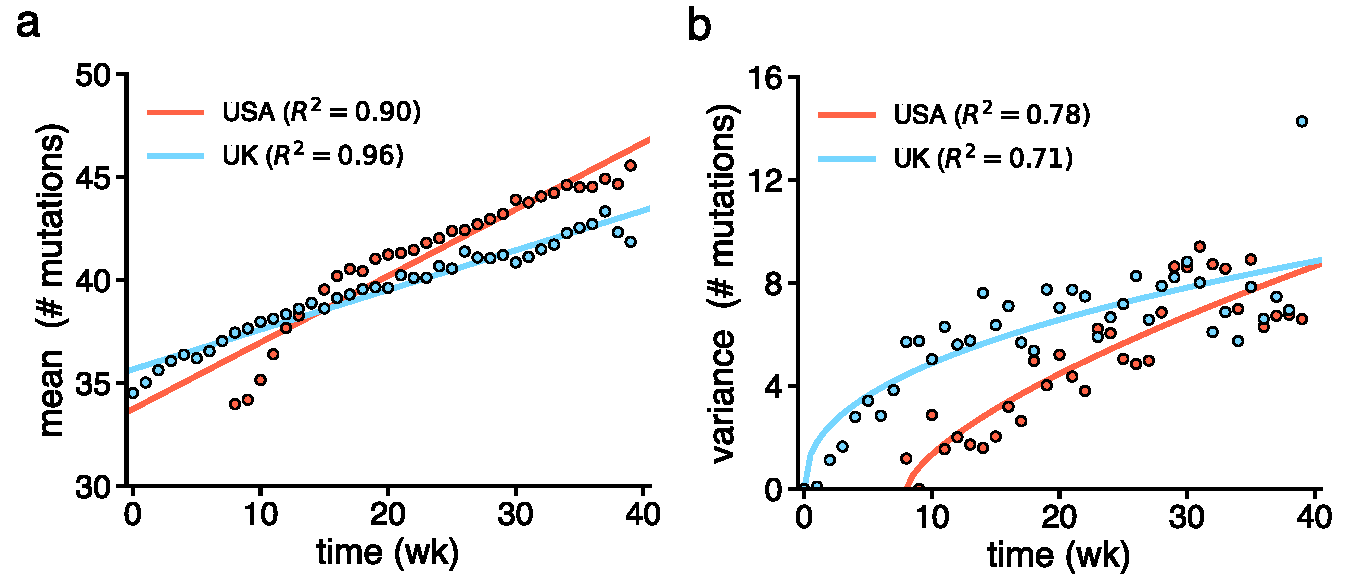
\includegraphics[width=0.95\textwidth]{assets/Ch3Fig2_horz.pdf}
    \caption{Mutational mean and variance over time in the SARS-CoV-2 Alpha variant genomes from UK and USA. a) Mean number of accumulated mutations. b) Scaled variance of the number of accumulated mutations. Points correspond to calculated values from the sequence dataset and lines to inferred molecular clock models.}\label{fig2:simulation_results}
\end{figure}

%CONCLUSIONS

\section{Conclusions}

Here, we present a high-throughput data-processing, open-source, user-friendly software, called PyEvoMotion, to study evolutionary motions under a statistical perspective provided a collection of genomic sequences. PyEvoMotion is designed to be flexible and customizable, offering a wide range of options for data analysis. Such statistical analysis is complementary to phylogenetic tree reconstructions and molecular assays that measure the impact of key mutations \cite{Mlcochova2021}. 

Nonetheless, our work presents some limitations. In the models, the evolution rate is assumed constant, despite it can vary with time if lineages with higher fitness emerge and even be non-linear if adaptation is the dominant process \cite{tenaillon2016}. This would require applying the date filter to limit the analysis to a subset of sequences, as we did to obtain the results shown in Figure~\ref{fig2:simulation_results}. Moreover, this statistical approach fails to provide meaningful insight if the collection of sequences is not sufficiently large and does not span in time.

In addition to virus evolution, PyEvoMotion might be used to study the tempo and mode of accumulation of mutations in bacteria \cite{tenaillon2016} or in cancer cells \cite{borgsmuller2023}. Understanding the dynamics of these rapidly evolving biological entities might have biomedical implications.

\section*{Data availability}
The open source software is available on GitHub at \href{https://github.com/luksgrin/PyEvoMotion}{\texttt{https://github.com/luksgrin/PyEvoMotion}} and on SourceForge at \href{https://sourceforge.net/projects/pyevomotion}{\texttt{https://sourceforge.net/projects/pyevomotion}}. Genomic data used in the validation were extracted from the GISAID database (\href{https://www.gisaid.org}{\texttt{https://www.gisaid.org}}) and are available on SourceForge.

\vfill

\pagebreak

\bibliographystyle{assets/rodrigostyle}
\bibliography{references/chapter3references}